\section{mr::distances::Type Struct Reference}
\label{structmr_1_1distances_1_1Type}\index{mr::distances::Type@{mr::distances::Type}}
{\tt \#include $<$mr\-Distances.h$>$}

Inheritance diagram for mr::distances::Type::\begin{figure}[H]
\begin{center}
\leavevmode
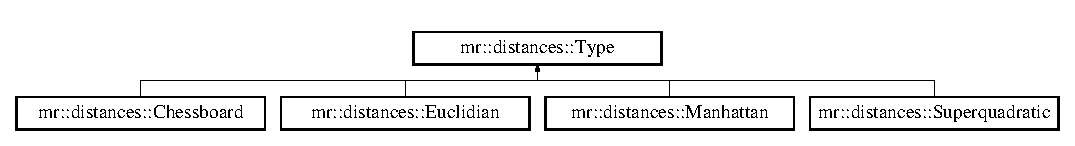
\includegraphics[height=1.51351cm]{structmr_1_1distances_1_1Type}
\end{center}
\end{figure}
\subsection*{Public Member Functions}
\begin{CompactItemize}
\item 
virtual mi\-Scalar {\bf operator()} (const {\bf vector} \&d) const=0
\item 
virtual mi\-Scalar {\bf operator()} (const {\bf vector} \&d, const {\bf vector} \&s) const=0
\end{CompactItemize}


\subsection{Detailed Description}
Different functors that can be used to measure common distance measurements. 



\subsection{Member Function Documentation}
\index{mr::distances::Type@{mr::distances::Type}!operator()@{operator()}}
\index{operator()@{operator()}!mr::distances::Type@{mr::distances::Type}}
\subsubsection{\setlength{\rightskip}{0pt plus 5cm}virtual mi\-Scalar mr::distances::Type::operator() (const {\bf vector} \& {\em d}, const {\bf vector} \& {\em s}) const\hspace{0.3cm}{\tt  [pure virtual]}}\label{structmr_1_1distances_1_1Type_a1}




Implemented in {\bf mr::distances::Euclidian} {\rm (p.\,\pageref{structmr_1_1distances_1_1Euclidian_a1})}, {\bf mr::distances::Manhattan} {\rm (p.\,\pageref{structmr_1_1distances_1_1Manhattan_a1})}, {\bf mr::distances::Chessboard} {\rm (p.\,\pageref{structmr_1_1distances_1_1Chessboard_a1})}, and {\bf mr::distances::Superquadratic} {\rm (p.\,\pageref{structmr_1_1distances_1_1Superquadratic_a1})}.\index{mr::distances::Type@{mr::distances::Type}!operator()@{operator()}}
\index{operator()@{operator()}!mr::distances::Type@{mr::distances::Type}}
\subsubsection{\setlength{\rightskip}{0pt plus 5cm}virtual mi\-Scalar mr::distances::Type::operator() (const {\bf vector} \& {\em d}) const\hspace{0.3cm}{\tt  [pure virtual]}}\label{structmr_1_1distances_1_1Type_a0}




Implemented in {\bf mr::distances::Euclidian} {\rm (p.\,\pageref{structmr_1_1distances_1_1Euclidian_a0})}, {\bf mr::distances::Manhattan} {\rm (p.\,\pageref{structmr_1_1distances_1_1Manhattan_a0})}, {\bf mr::distances::Chessboard} {\rm (p.\,\pageref{structmr_1_1distances_1_1Chessboard_a0})}, and {\bf mr::distances::Superquadratic} {\rm (p.\,\pageref{structmr_1_1distances_1_1Superquadratic_a0})}.

The documentation for this struct was generated from the following file:\begin{CompactItemize}
\item 
{\bf mr\-Distances.h}\end{CompactItemize}
